\documentclass[a4paper]{article}

\def\nterm {April}
\def\nyear {2024}
\def\nlecturer {Ryan Tibshirani}
\def\ncourse {Convex Optimization: Fall 2019}

../header.tex

\begin{document}
\maketitle
{\small
\noindent\textbf{Course Information}\\ 
\indent \textbf{Instructor:} \textcolor{blue}{\href{https://www.stat.berkeley.edu/~ryantibs/index.html}{\nlecturer}} \\
\indent\textbf{Homepage:} \textcolor{blue}{\href{https://www.stat.cmu.edu/~ryantibs/convexopt/}{Machine Learning 10-725}} \\
\indent\textbf{Teaching:} Carnegie Mellon University \\

\vspace{10pt}
\noindent\textbf{Schedule}\\
\indent This course is divided into five parts: 
\begin{enumerate}
    \item \textbf{Theory I: Fundamentals}
    \begin{itemize}
        \item Introduction
        \item 
    \end{itemize}
    \item \textbf{Algorithms I: First-order methods}
    \item \textbf{Theory II: Duality and optimality}
    \item \textbf{Algorithms II: Second-order methods}
    \item \textbf{Advanced topics}
\end{enumerate}

\tableofcontents

\setcounter{section}{-1}
\section{Introduction}
\begin{defi}[Convex set]
    $C \subseteq \R^n$ such that 
    \[
        x, y \in C \Longrightarrow  tx + (1-t)y \in C,\text{\ for\ all}\ 0 \leq t \leq 1 
    \]
\end{defi}

% \begin{center}
%     \begin{tikzpicture}
%         % convex set
%         \coordinate (A) at (-4,0);
%         \coordinate (B) at (-3,0.2);
%         \coordinate (C) at (-2.5,1.23);
%         \coordinate (D) at (-4,2);
%         \coordinate (E) at (-5,1.2);
%         \draw (A) -- (B) -- (C) -- (D) -- (E) -- cycle;
%         \filldraw[fill=gray!30] (A) -- (B) -- (C) -- (D) -- (E) -- cycle;

%         % non-convex set
%         \draw (0, 0) .. controls (-0.1, 1.5) and (1.8,2) .. (2, 1);
%         \draw (0, 0) .. controls (1, 0.2) and (0.5,-0.1) .. (1, 1);
%         \draw (1, 1) .. controls (2, 0.8) and (1.6,0.4) .. (2, 1);

%         \end{tikzpicture}
% \end{center}
\begin{figure}[htbp] 
  \centering 
  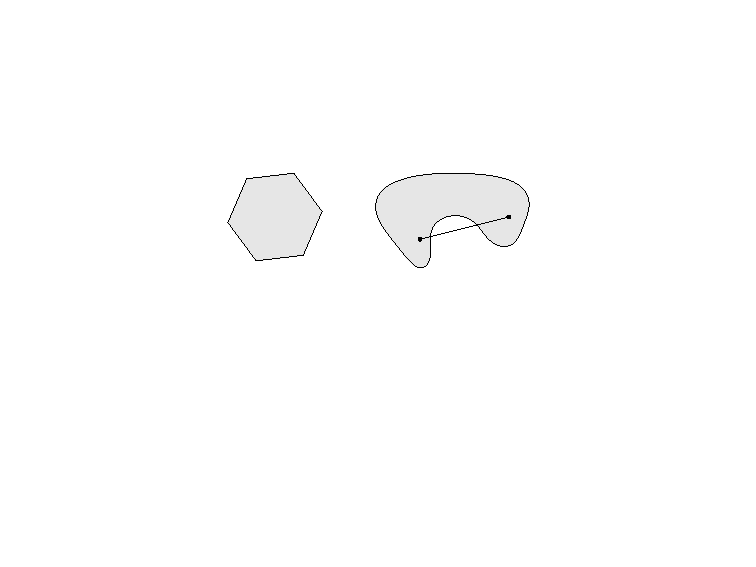
\includegraphics[width=0.6\textwidth]{img/convex_set.pdf} 
\end{figure}


\begin{defi}[Convex function]
    $f: \R^n \rightarrow \R$ such that $\dom (f) \subseteq \R^n$ convex, and 
    \[
        f(tx + (1-t)y) \leq tf(x) + (1-t)f(y),\text{\ for\ all}\ 0 \leq t \leq 1 
    \]
    and all $x, y \in \dom (f)$
\end{defi}

\begin{center}
    \begin{tikzpicture}
      \draw (0.27, 0.5) -- (3, 1);
      \draw (0, 1) .. controls (1,-1) .. (3.5, 1.5);
      \node  at (0.27, 0.5) [circ] {}; 
      \node at (0.27, 0.5) [left] {$(x, f(x))$};
      \node at (3, 1) [circ] {};
      \node at (3, 1) [right] {$(y, f(y))$};
    \end{tikzpicture}
\end{center}

\begin{defi}[Optimization problem] 
    \begin{align*}
        \min _{x \in D} & \quad f(x) \\
        \text { subject to } &\quad g_{i}(x) \leq 0, \ i=1, \ldots, m \\
        &\quad h_{j}(x)=0, \ j=1, \ldots, r
    \end{align*}
\end{defi}
Here $D = \dom (f) \cap \bigcap_{i=1}^{m} \dom (g_{i}) \cap \bigcap_{j=1}^{r} \dom(h_j)$, common domain of all functions.

\begin{figure}[htbp] 
  \centering 
  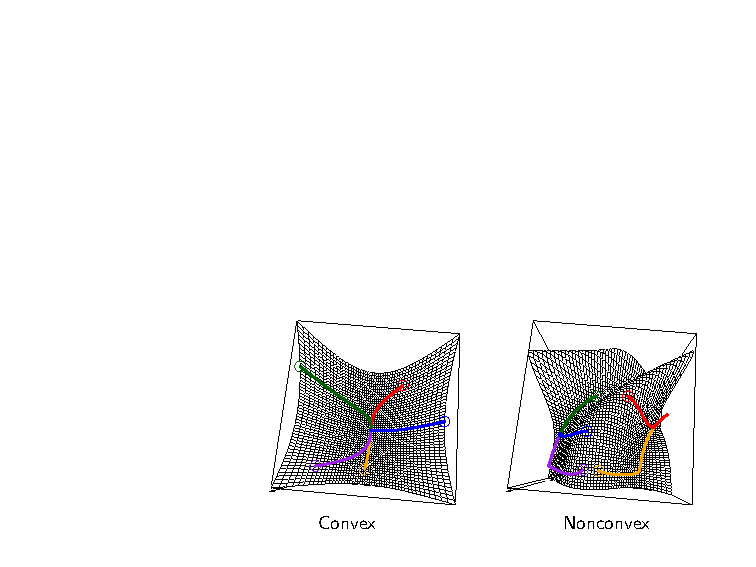
\includegraphics[width=0.6\textwidth]{img/convex_vs_nonconvex.pdf} 
\end{figure}

This is a \textbf{convex optimization problem} provided the functions $f$ and $g_i, i=1,\ldots,m$ are convex, and  $h_j, j=1,\ldots,r$ are affine:
\[
    h_j (x) = a_{j}^{T}x + b_j, \quad j =1,\ldots,r
\]

For convex optimization problem, \textbf{local minima are global minima}.
Formally, if $x$ is feasible---$x \in D$, and satisfies all constraints and minimizes $f$ in a local neighborhood,
\[
    f(x) \leq f(y) \text{\ for \ all \ feasible} \ y, \ \left\lVert x -y \right\rVert_2 \leq \rho
\]
then
\[
    f(x) \leq f(y) \text{\ for \ all \ feasible} \ y
\]

\section{Differentiation}
We will first quickly go through basic notions of differentiation and integration. You should already be familiar with these from A levels or equivalent.

\subsection{Differentiation}
\begin{defi}[Derivative of function]
  The \emph{derivative} of a function $f(x)$ with respect to $x$, interpreted as the rate of change of $f(x)$ with $x$, is
  \[
    \frac{\d f}{\d x} = \lim_{h\to 0} \frac{f(x + h) - f(x)}{h}.
  \]
  A function $f(x)$ is differentiable at $x$ if the limit exists (i.e.\ the left-hand and right-hand limits are equal).
\end{defi}

\begin{eg}
  $f(x)=|x|$ is not differentiable at $x = 0$ as $\lim\limits_{h\to 0^+} \frac{|h| - |0|}{h}= 1$ and $\lim\limits_{h\to 0^-} \frac{|h| - |0|}{h}= -1$.
\end{eg}

\begin{notation}
  We write $\frac{\d f}{\d x} = f'(x) = \frac{\d}{\d x} f(x)$. Also, $\frac{\d}{\d x}\left(\frac{\d}{\d x} f(x)\right) = \frac{\d^2}{\d x^2} f(x) = f''(x)$.

  Note that the notation $f'$ represents the derivative with respect to the argument. For example, $f'(2x) = \frac{\d f}{\d (2x)}$
\end{notation}

\subsection{Small \texorpdfstring{$o$}{o} and big \texorpdfstring{$O$}{O} notations}
\begin{defi}[$O$ and $o$ notations]\leavevmode
  \begin{enumerate}
    \item ``$f(x) = o(g(x))$ as $x\to x_0$'' if $\lim\limits_{x\to x_0} \frac{f(x)}{g(x)} = 0$. Intuitively, $f(x)$ is much smaller than $g(x)$.
    \item ``$f(x) = O(g(x))$ as $x\to x_0$'' if $\frac{f(x)}{g(x)}$ is bounded as $x\to x_0$. Intuitively, $f(x)$ is about as big as $g(x)$.

      Note that for $f(x) = O(g(x))$ to be true, $\displaystyle \lim_{x\to x_0} \frac{f(x)}{g(x)}$ need not exist.
  \end{enumerate}
  Usually, $x_0$ is either $0$ or infinity. Clearly, we have $f(x)=o(g(x))$ implies $f(x) = O(g(x))$.
\end{defi}
Note that this is an abuse of notation. We are not really saying that $f(x)$ is ``equal'' to $o(g(x))$, since $o(g(x))$ itself is not a function. Instead, $o(g(x))$ represents a \emph{class} of functions (namely functions that satisfy the property above), and we are saying that $f$ is in this class. Technically, a better notation might be $f(x) \in o(g(x))$, but in practice, writing $f(x) = o(g(x))$ is more common and more convenient.

\begin{eg}\leavevmode
  \begin{itemize}
    \item $x=o(\sqrt{x})$ as $x\to 0$ and $\sqrt{x} = o(x)$ as $x\to \infty$.
    \item $\sin 2x = O(x)$ as $x\to 0$ as $\sin \theta \approx \theta$ for small $\theta$.
    \item $\sin 2x = O(1)$ as $x\to \infty$ even though the limit does not exist.
  \end{itemize}
\end{eg}

This notation will frequently be used in calculus. For example, if we want to ignore all terms second order in $x$ in an expression, we can write out the first order terms and then append $+O(x^2)$. In particular, we can use it to characterize derivatives in a different way.
\begin{prop}
  \[
    f(x_0 + h) = f(x_0) + f'(x_0)h + o(h)
  \]
\end{prop}

\begin{proof}
  We have
  \[
    f'(x_0) = \frac{f(x_0 + h) - f(x_0)}{h} + \frac{o(h)}{h}
  \]
  by the definition of the derivative and the small $o$ notation. The result follows.
\end{proof}

\subsection{Methods of differentiation}
\begin{thm}[Chain rule]
  Given $f(x) = F(g(x))$, then
  \[
    \frac{\d f}{\d x} = \frac{\d F}{\d g}\frac{\d g}{\d x}.
  \]
\end{thm}

\begin{proof}
  Assuming that $\frac{\d g}{\d x}$ exists and is therefore finite, we have
  \begin{align*}
    \frac{\d f}{\d x} &= \lim_{h\to 0}\frac{F(g(x + h)) - F(g(x))}{h}\\
    &= \lim_{h\to 0}\frac{F[g(x) + hg'(x) + o(h)] - F(g(x))}{h}\\
    &= \lim_{h\to 0}\frac{F(g(x)) + (hg'(x) + o(h))F'(g(x)) + o(hg'(x) + o(h)) - F(g(x))}{h}\\
    &= \lim_{h\to 0}g'(x)F'(g(x)) + \frac{o(h)}{h}\\
    &= g'(x)F'(g(x))\\
    &= \frac{\d F}{\d g}\frac{\d g}{\d x}\qedhere
  \end{align*}
\end{proof}

\begin{thm}[Product Rule]
  Give $f(x) = u(x)v(x)$. Then
  \[
    f'(x) = u'(x)v(x) + u(x)v'(x).
  \]
\end{thm}

\begin{thm}[Leibniz's Rule]
  Given $f = uv$, then
  \[
    f^{(n)}(x) = \sum_{r = 0}^n \binom{n}{r}u^{(r)}v^{(n - r)},
  \]
  where $f^{(n)}$ is the n-th derivative of $f$.
\end{thm}

\subsection{Taylor's theorem}
\begin{thm}[Taylor's Theorem]
  For $n$-times differentiable $f$, we have
  \[
    f(x + h) = f(x) + hf'(x) + \frac{h^2}{2!}f''(x) + \cdots + \frac{h^n}{n!}f^{(n)}(x) + E_n,
  \]
  where $E_n = o(h^{n})$ as $h\to 0$. If $f^{(n+1)}$ exists, then $E_n = O(h^{n+1})$.
\end{thm}
Note that this only gives a local approximation around $x$. This does not necessarily tell anything about values of $f$ far from $x$ (but sometimes does).

An alternative form of the sum above is:
\[
  f(x) = f(x_0) + (x-x_0)f'(x_0) + \cdots + \frac{(x-x_0)^n}{n!}f^{(n)}(x_0) + E_n.
\]
When the limit as $n\to \infty$ is taken, the Taylor series of $f(x)$ about the point $x = x_0$ is obtained.

\subsection{L'Hopital's rule}
\begin{thm}[L'Hopital's Rule]
  Let $f(x)$ and $g(x)$ be differentiable at $x_0$, and $\displaystyle \lim_{x\to x_0}f(x) = \lim_{x\to x_0}g(x) = 0$. Then
  \[
    \lim_{x\to x_0} \frac{f(x)}{g(x)} = \lim_{x\to x_0} \frac{f'(x)}{g'(x)}.
  \]
\end{thm}
\begin{proof}
  From the Taylor's Theorem, we have $f(x) = f(x_0) + (x - x_0)f'(x_0) + o(x - x_0)$, and similarly for $g(x)$. Thus
  \begin{align*}
    \lim_{x\to x_0} \frac{f(x)}{g(x)} &= \lim_{x\to x_0} \frac{f(x_0) + (x - x_0)f'(x_0) + o(x - x_0)}{g(x_0) + (x - x_0)g'(x_0) + o(x - x_0)}\\
    &= \lim_{x\to x_0} \frac{f'(x_0) + \frac{o(x-x_0)}{x-x_0}}{g'(x_0) + \frac{o(x-x_0)}{x-x_0}}\\
    &= \lim_{x\to x_0} \frac{f'(x)}{g'(x)}\qedhere
  \end{align*}
\end{proof}

\end{document}